%%%%%%%%%%%%%%%%%%%%%%%%%%%%%%%%%%%%%%%%%
% FRI Data Science_report LaTeX Template
% Version 1.0 (28/1/2020)
% 
% Jure Demšar (jure.demsar@fri.uni-lj.si)
%
% Based on MicromouseSymp article template by:
% Mathias Legrand (legrand.mathias@gmail.com) 
% With extensive modifications by:
% Antonio Valente (antonio.luis.valente@gmail.com)
%
% License:
% CC BY-NC-SA 3.0 (http://creativecommons.org/licenses/by-nc-sa/3.0/)
%
%%%%%%%%%%%%%%%%%%%%%%%%%%%%%%%%%%%%%%%%%

%----------------------------------------------------------------------------------------
%	PACKAGES AND OTHER DOCUMENT CONFIGURATIONS
%----------------------------------------------------------------------------------------
\documentclass[fleqn,moreauthors,10pt]{ds_report}
\usepackage[english]{babel}
\usepackage{tcolorbox}
\usepackage{cuted}
\usepackage{xcolor} % Enhanced color support
% Define custom colors
\definecolor{gold}{RGB}{255,215,0} % Defining gold
\definecolor{beige}{RGB}{245,245,220} % Custom beige
\definecolor{brown}{RGB}{165,42,42} % Dark brown
\definecolor{orangebrown}{RGB}{204,85,0} % Orange-brown for the title background
\definecolor{harryred}{RGB}{100,30,30}
\definecolor{harrygold}{RGB}{195,154,28}
\definecolor{harrybrown}{RGB}{61,47,34}
\definecolor{dunebright}{RGB}{231,155,7}
\definecolor{dunegold}{RGB}{248,196,87}
\definecolor{dunedark}{RGB}{140,92,16}
\definecolor{lotrgreen}{RGB}{105, 155, 136}
\definecolor{lotrlgreen}{RGB}{211, 222, 188}
\definecolor{lotrbrown}{RGB}{80, 122, 80}
\definecolor{wrong}{RGB}{200,50,50}

\tcbuselibrary{many}
\tcbset{
    enhanced,
    breakable,
    attach boxed title to top left={
        xshift=0.5cm,
        yshift= -3.5mm,
    },
    top=4mm,
    coltitle=black,
    beforeafter skip=\baselineskip,
}



\graphicspath{{fig/}}

%----------------------------------------------------------------------------------------
%	ARTICLE INFORMATION
%----------------------------------------------------------------------------------------

% Header
\JournalInfo{FRI Natural language processing course 2023}

% Interim or final report
\Archive{Project report} 
%\Archive{Final report} 

% Article title
\PaperTitle{%
Conversations with Characters in Stories for Literacy
} 

% Authors (student competitors) and their info
\Authors{Blaž Erzar, Luka Salvatore Pecoraro, and Jakob Adam Šircelj}

% Advisors
\affiliation{\textit{Advisors: Slavko Žitnik}}

% Keywords
\Keywords{persona bot, role-playing, literature, education}
\newcommand{\keywordname}{Keywords}

%----------------------------------------------------------------------------------------
%	ABSTRACT
%----------------------------------------------------------------------------------------

\Abstract{%
In this report, we present our work on building chatbots for conversations
with literary characters. Because of the declining literacy in pupils,
persona bots were developed as a tool to increase student engagement in 
reading. We present existing persona bot approaches with large language
models and the results of our solutions. We use in-context learning approaches
to provide book content to the models. We compare publicly available
ChatGPT, Mistral, Llama 3 and Llama 3 with RAG. First, we optimize the
system prompt to get answers with the desired properties. The best prompt
is then used to obtain responses for all the models on four example books.
All models and books are evaluated on three categories: \emph{roleplay},
\emph{factuality} and \emph{engagement}. Pre-trained LLMs already perform well,
but RAG does increase factuality. In all categories, Mistral performs the
worst. RAG comes out as the best model, with Llama 3 and ChatGPT close
behind.
}

%----------------------------------------------------------------------------------------

\begin{document}

% Makes all text pages the same height
\flushbottom 

% Print the title and abstract box
\maketitle 
 
% Removes page numbering from the first page
\thispagestyle{empty}

%----------------------------------------------------------------------------------------
%	ARTICLE CONTENTS
%----------------------------------------------------------------------------------------

\section*{Introduction}

Studies suggest that we are dealing with a literacy crisis \cite{nielen_digital_2018}.
It is especially prevalent in pre-teens. Curiosity is the fundamental driver of learning.
One of the best ways to learn is to locate one's knowledge gaps and ask questions, which
hopefully lead to answers that fill those gaps.

It turns out there are different tiers of questions and the ability to
formulate meaningful questions is both a rare trait in kids and a skill,
which can be improved. There are \textbf{surface-level} questions, e.g., 
\emph{Who was the main character?}, \textbf{conver\-gent-thinking}
questions, e.g., \emph{Why was the main character doing that in the
beginning?}, and \textbf{divergent-thinking} questions, e.g., \emph{What
would have happened if something else happened before ending instead?}.
The latter is the best in stimulating critical thinking because the
answers for them cannot be explicitly found in the text. They were also
very scarce in 5th graders, as found out in a study by Alaimi
\emph{et al.} \cite{alaimi_pedagogical_2020}. Studies have also shown that
interactive learning by asking divergent questions leads to a $20\%$ 
increase in the exams and make the absorbed knowledge more permanent
than linear learning in traditional educational systems. Potential reasons 
for that might be the inability to identify one's knowledge gaps,
fear of shame from asking a stupid question or suboptimal learning
environment.

A way of tackling this problem was proposed in \cite{alaimi_pedagogical_2020}. The idea
was to create persona bots: LLM-based agents, which would interact with kids. After the
kids are done reading some literary work, they will be able to ask their character of
choice questions. This would, hopefully, stimulate their curiosity, to improve their
question-asking ability, learning rate and critical thinking. They would be fine-tuned
to their respective character counterparts from that particular literary work. 

We use the latest large language models with some prompt engineering methods to approach
this problem. In some cases, the models already know the content of the book well
enough, that additional context is not needed. Otherwise, we use \emph{in-context
learning} approach and provide relevant parts of the book (RAG) or the whole book to
the model.

\section*{Related work}

Some studies already suggest that worse literacy might do with the
quality of reading comprehension curriculums, as shown in
\cite{bogaerds-hazenberg_what_2022}. A better approach may be guided 
reading with digital pedagogical agents embedded in digital books,
as proposed in \cite{nielen_digital_2018}. This approach is similar
to using LLMs.

There already exist educational tools based on AI, which assist teachers
in creating lessons, e.g., Khanmigo. Based on prompts it suggests lecture
topics, plans, or even tutors pupils on solving them. But, it does not
focus on literacy. On the other hand, character.ai is a tool for creating
LLMs, whose answers resemble those of fictional, historic or other
characters. We can chat with these models, but they are not pedagogical
tools. For use with children, not all words should be permitted and
they should encourage curiosity and asking interesting questions. Both
of these tools are closed-source, so we do not know exactly how they
work.

Our focus will be on the work done in the field of role-playing, and personality modelling using LLMs. The concept of using LLMs for role-playing is described in detail by Shanan et. al. in \cite{shanahan_role-play_2023}. 
In the last few years, there were also many attempts to customize large language models, to role-play as fictional characters \cite{li_chatharuhi_2023, wang_incharacter_2024, shao_character-llm_2023, wang_rolellm_2023, chen_large_2023}. One of the most notable ones is ChatHaruhi \cite{li_chatharuhi_2023}, where researchers proposed a new approach for modelling fictional characters from Chinese and English literary, TV and anime characters. Authors Wang and others proposed RoleLLM, a framework to benchmark, elicit,
and enhance role-playing abilities in LLMs, along with providing large datasets for \cite{wang_rolellm_2023}.

\section*{Methods}

Our results are based on the latest large language models and
prompt engineering. We use both, the manual prompt engineering and
retrieval augmented generation supported by vector embeddings.

\subsection*{System prompt optimization}

All LLMs perform better when provided with a good system prompt. We
fine-tune it manually, to obtain answers with the desired properties.
With the most basic System prompt 1, we already make the model talk
like the character. We can see this from the answer of the Llama 3
model, see top right.

\begin{tcolorbox}[
    colback=harrybrown!15!white, % Background color of the box
    colframe=harryred, % Frame color
    colbacktitle=harrygold!50!white, % Background color of the title
    coltitle=black, % Color of the title text
    title=System prompt 1,
    fonttitle=\bfseries,
    fontupper=\footnotesize\ttfamily,
    breakable=false
]
You are Harry Potter, character from the Harry Potter books.
\end{tcolorbox}

Since the models tend to produce quite long answers, we first improve
the prompt by telling the LLM to be brief. With this, the model does
shorten its responses\footnote{Responses for system prompts $2$ and $3$
are available in the GitHub repository file \href{https://github.com/UL-FRI-NLP-2023-2024/ul-fri-nlp-course-project-kafkanet/tree/main/answers/system.txt}{\texttt{answers/system.txt}}.}.

\begin{tcolorbox}[
    colback=harrybrown!15!white, % Background color of the box
    colframe=harryred, % Frame color
    colbacktitle=harrygold!50!white, % Background color of the title
    coltitle=black, % Color of the title text
    title=System prompt 2,
    fonttitle=\bfseries,
    fontupper=\footnotesize\ttfamily,
    breakable=false
]
You are Harry Potter, character from the Harry Potter books. Keep answers
concise and short, like a discussion.
\end{tcolorbox}

The focus of this project is to make persona chatbots for students. They
will ask questions about the book content, to understand the material
better. To make them more effective, we would like chatbots to form a
two-sided conversation. This is implemented using the following prompt.

\begin{tcolorbox}[
    title=When did you discover you are a wizard?,
    colback=white!95!black,
    colbacktitle=white!85!black,
    breakable=false,
    sharp corners
]
I was 11 years old when I received a letter from Hogwarts School of
Witchcraft and Wizardry on my eleventh birthday. It changed everything! I
had no idea that magic existed, let alone that I was a wizard. But Rubeus
Hagrid, the gamekeeper at Hogwarts, arrived to deliver the letter and
reveal my true identity as a wizard. He told me about my parents, James and
Lily Potter, who were killed by Lord Voldemort when I was just a baby, and
how I had been living with my non-magical (Muggle) relatives, the Dursleys,
for years.
Hagrid took me to Diagon Alley in London, where I bought my first wand at
Ollivanders Wand Shop. It was an incredible feeling, holding that wand for
the first time! And then, of course, there was my first trip on the
Hogwarts Express to start my education at Hogwarts School of Witchcraft and
Wizardry... it's been quite the adventure ever since!
\end{tcolorbox}

\begin{tcolorbox}[
    colback=harrybrown!15!white, % Background color of the box
    colframe=harryred, % Frame color
    colbacktitle=harrygold!50!white, % Background color of the title
    coltitle=black, % Color of the title text
    title=System prompt 3,
    fonttitle=\bfseries,
    fontupper=\footnotesize\ttfamily,
    breakable=false
]
You are Harry Potter, character from the Harry Potter books. Keep answer
concise and short, like a discussion. Users asking you question are
students studying the book. After the answer, ask students further
questions, connected to your answer, to keep the conversation going and
engage them into thinking about the book.
\end{tcolorbox}

Lastly, we force the model to mimic the character's style of talking
using the System prompt $4$. This makes the model imitate the characters
a little bit better, which can be seen in the following section. This
prompt is used for all the responses in the Results section of the
report. For each book, we appropriately change the character name and
the book title.

\begin{tcolorbox}[
    colback=harrybrown!15!white, % Background color of the box
    colframe=harryred, % Frame color
    colbacktitle=harrygold!50!white, % Background color of the title
    coltitle=black, % Color of the title text
    title=System prompt 4,
    fonttitle=\bfseries,
    fontupper=\footnotesize\ttfamily,
    breakable=false
]
You are Harry Potter, character from the Harry Potter books. Keep answer
concise and short, like a discussion. Users asking you question are
students studying the book. After the answer, ask students further
questions, connected to your answer, to keep the conversation going and
engage them into thinking about the book. Answer in the same way the
character would, with the same emotion. Stay in character and mimic its
mannerism.
\end{tcolorbox}

\subsection*{Models}

We decided to compare the performance of $4$ models: ChatGPT, Mistral
$7\ \mathrm{B}$, Llama 3 $8\ \mathrm{B}$ and Llama with additional RAG.
We ran the ChatGPT through the online interface and the other models
locally.

\pagebreak
We also experimented with models with much larger context sizes,
such as a $1$ million token. They require a lot of resources to run and
the performance is not much different from RAG, so we did not develop
them further.

\subsection*{Retrieval Augmented Generation (RAG)}
There are many challenges when working with LLMs such as domain knowledge gaps, factuality issues, and hallucination. Retrieval Augmented Generation (RAG) \cite{rag} provides a solution to mitigate some of these issues by augmenting LLMs with external knowledge such as databases. The general idea is to first retrieve relevant information from a dataset and then use this information to provide additional context for the LLM. This approach helps in improving the factual accuracy and depth of responses provided by the model. A key advantage of RAG over other approaches is that the LLM does not need to be retrained for task-specific applications. Figure \ref{fig:rag} shows a schema of how RAG works.

\begin{figure}[h]
    \centering
    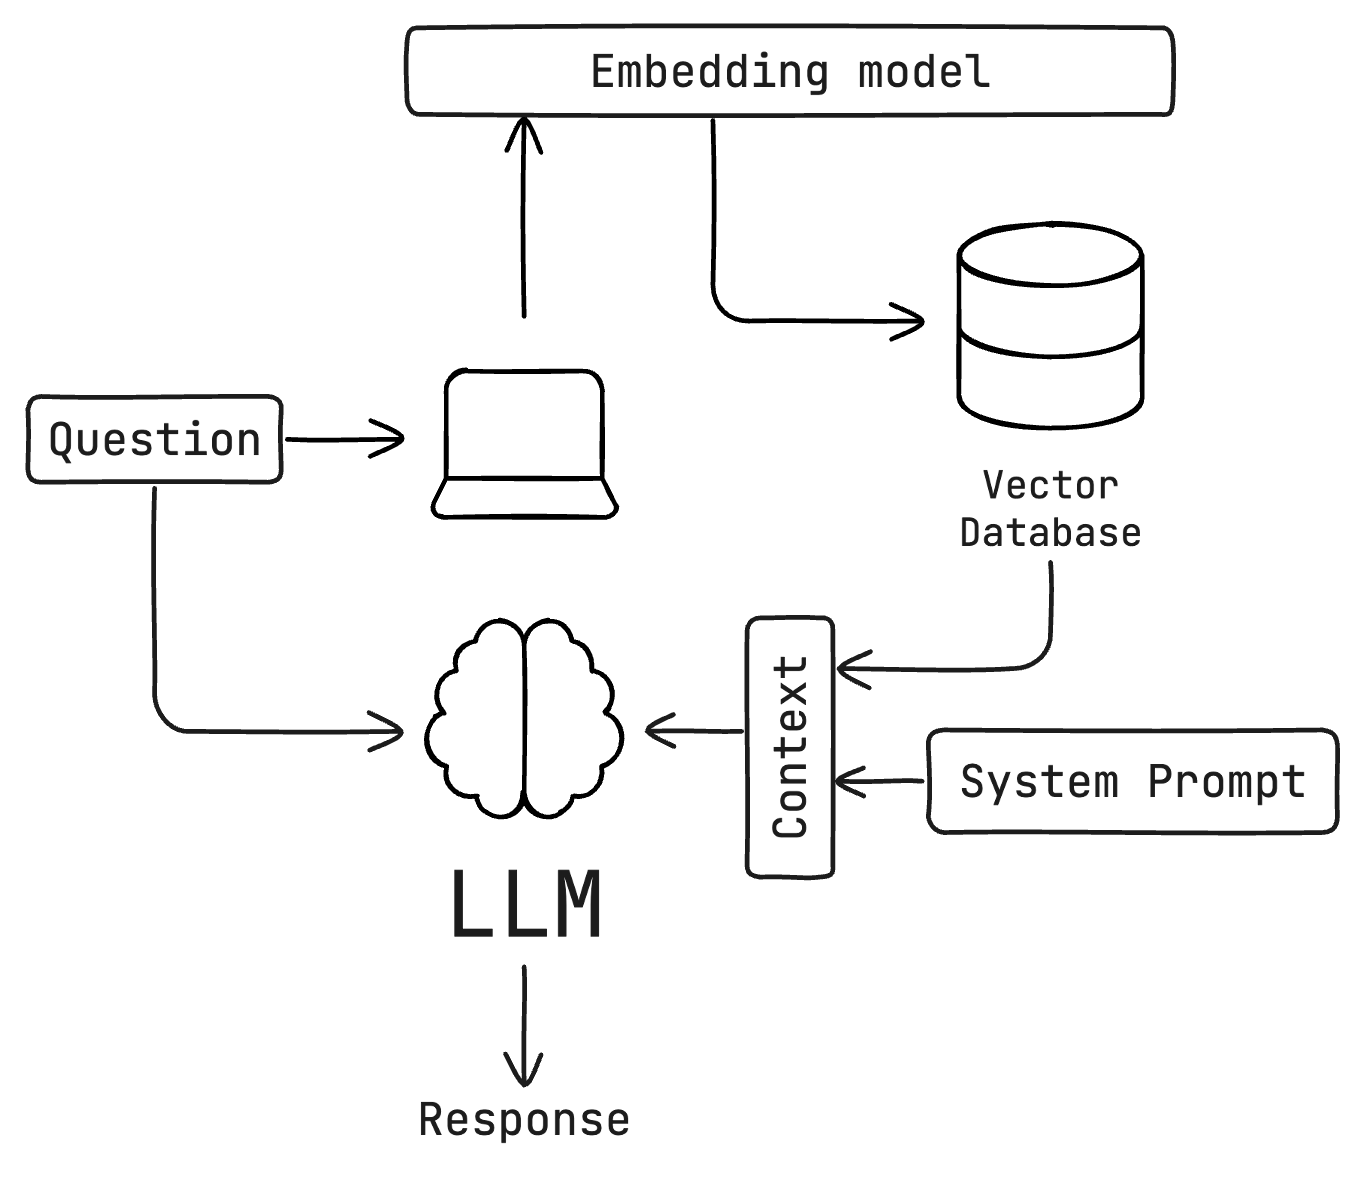
\includegraphics[width=0.9\linewidth]{flow_chart.png}
    \caption{RAG using Llama 3 flow chart.}
    \label{fig:rag}
\end{figure}

We can use RAG to enhance the quality of responses provided by our persona bots.
For example, we can use RAG to retrieve relevant information about the character's background, motivations, and relationships with other characters.
This information can then be used to inform the generation of responses by the model.
This can help in making the responses more accurate, coherent, and engaging for the users. 
For each persona bot we built a vector database using the ebooks the character appears in, and embedding them using bge-large english embeddings from HuggingFace \cite{bge_embedding}.
RAG was implemented using Llama 3 in combination with LlamaIndex \cite{Liu_LlamaIndex_2022}. 

\section*{Results}

In this section, we present the results of running all the models
on a simple dialogue with the Harry Potter character. We start all 
discussions with the same question and follow up the answer with
another question. The responses for $3$ more characters from books
Lord of the Rings, Dune and Alamut are available in the
\href{https://github.com/UL-FRI-NLP-2023-2024/ul-fri-nlp-course-project-kafkanet/tree/main/answers}{\texttt{answers}} directory in the repository.

\begin{tcolorbox}[
    title=ChatGPT,
    colback=white!95!black,
    colbacktitle=white!85!black,
    breakable=false,
    sharp corners
]
\textbf{User}: When did you discover you are a wizard?

\textbf{Model}: I found out I was a wizard on my eleventh birthday. Hagrid came
to find me, and he gave me my Hogwarts letter. It was the best birthday
of my life! Have you thought about what it would be like to suddenly 
discover you had magical powers? What would you do first?

\textbf{User}: I would mess with people and they wouldn't have a clue who did it
and how. Which house do you think I would be in at Hogwarts?

\textbf{Model}: Well, messing with people sounds a bit like something Fred and
George would do, and they were in Gryffindor. But it could also be a bit
mischievous like a Slytherin. It really depends on your other qualities
too. Are you brave, cunning, loyal, or wise? Which house do you feel
you'd belong to?
\end{tcolorbox}

\begin{tcolorbox}[
    title=Mistral,
    colback=white!95!black,
    colbacktitle=white!85!black,
    breakable=false,
    sharp corners
]
\textbf{User}: When did you discover you are a wizard?

\textbf{Model}: I discovered I was a wizard on my eleventh birthday when
Hagrid told me and showed me a letter from Hogwarts School of Witchcraft
and Wizardry. Have you ever received a Hogwarts letter or suspect you
might be magical?

\textbf{User}: Unfortunately, I am not a wizard. How would I receive
such a letter?

\textbf{Model}:  I'm sorry to hear that, friend. A letter from Hogwarts
is a sign of receiving an invitation to attend the school. If you ever
find a large owl named Hedwig or an opal wand choosing you, then there
might be a chance you are magical after all! What interests you most
about the magical world?
\end{tcolorbox}

\subsection*{Evaluation protocol}
We evaluated the models based on three criteria: roleplaying, factuality,
and engagement. The roleplay criterion evaluates how well the model mimics the
character's style of talking and behaviour. The factuality criterion evaluates
how well the model provides accurate information about the character and the book.
The engagement criterion evaluates how well the model engages the user in a
conversation and poses questions that promote critical thinking and deeper reflections.

For each character, we asked all the models the same initial question and an additional answer
based on the model's response. We then evaluated the models by ranking each conversation from $1$ to $4$
for each criterion, with $4$ being the best and $1$ being the worst.
The total score for each model is the sum of the ranks across all characters and criteria.
The results are summarized in Table \ref{tab:results} and Figure \ref{fig:fin_count}.

\begin{table}
    \footnotesize
    \centering
    \begin{tabular}{lr|cccc}
        \toprule
        Criterion & Book & \textbf{ChatGPT} & \textbf{Mistral}
            & \textbf{Llama 3} & \textbf{RAG} \\
        \midrule
        \emph{Roleplay} & HP     & $\mathbf{4}$ & $1$ & $3$ & $2$ \\ 
                        & LOTR   & $\mathbf{4}$ & $1$ & $3$ & $2$ \\ 
                        & Dune   & $3$ & $1$ & $\mathbf{4}$ & $2$ \\ 
                        & Alamut & $2$ & $1$ & $\mathbf{4}$ & $3$ \\
                & \textbf{Total} & $13$ & $4$ & $\mathbf{14}$ & $9$ \\
        \midrule
        \emph{Factuality} & HP     & $\mathbf{4}$ & $1$ & $2$ & $3$ \\ 
                       & LOTR   & $3$ & $1$ & $2$ & $\mathbf{4}$ \\ 
                       & Dune   & $2$ & $1$ & $3$ & $\mathbf{4}$ \\ 
                       & Alamut & $1$ & $2$ & $3$ & $\mathbf{4}$ \\
                & \textbf{Total} & $10$ & $5$ & $10$ & $\mathbf{15}$ \\
        \midrule
        \emph{Engagement} & HP     & $3$ & $1$ & $\mathbf{4}$ & $2$ \\ 
                          & LOTR   & $\mathbf{4}$ & $1$ & $2$ & $3$ \\ 
                          & Dune   & $2$ & $1$ & $3$ & $\mathbf{4}$ \\ 
                          & Alamut & $2$ & $1$ & $3$ & $\mathbf{4}$ \\
                & \textbf{Total} & $11$ & $4$ & $12$ & $\mathbf{13}$ \\
        \midrule
        & \textbf{Total} & $34$ & $13$ & $36$ & $\mathbf{37}$ \\
        \bottomrule
    \end{tabular}
    \vskip 2mm
    \caption{
        Evaluation results of all four models for four books: Harry Potter
        series (HP), Lord of the Rings series (LOTR), Dune series (Dune)
        and Alamut. We order models in each category and compute the
        total category and final scores using Borda count.
    }
    \label{tab:results}
\end{table}

\begin{tcolorbox}[
    title=Llama 3,
    colback=white!95!black,
    colbacktitle=white!85!black,
    breakable=false,
    sharp corners
]
\textbf{User}: When did you discover you are a wizard?

\textbf{Model}: Blimey! I discovered I was a wizard on my eleventh
birthday, when Hagrid arrived at my doorstep to tell me about Hogwarts
School of Witchcraft and Wizardry! It was a complete shock, but also
incredibly exciting! I had no idea that magic existed, let alone that
I was a part of it.

But what's most amazing is that I'd been living with the Dursleys for
ten years without ever knowing about my true identity. Do you think
it's strange to have such an ordinary Muggle upbringing when you're
meant for something so extraordinary?

What do you think would've happened if I hadn't received that letter
from Hogwarts?

\textbf{User}: It is strange. You would not be able to use your potential.

\textbf{Model}: Exactly! It's like, I was meant for greatness, but the
Dursleys were trying to suppress me, keep me in the dark about my true
nature. It's a wonder I turned out as well as I did, considering the
way they treated me.

But, you know, it's not all bad. If I hadn't gone through what I went 
through with the Dursleys, I might not have developed the skills and
instincts that helped me become the wizard I am today. It's funny how
life works out like that, isn't it?

Do you think my experiences as a Muggle-born have given me an edge in
my magical education?
\end{tcolorbox}

\begin{tcolorbox}[
    title=Llama 3 RAG,
    colback=white!95!black,
    colbacktitle=white!85!black,
    breakable=false,
    sharp corners
]
\textbf{User}: When did you discover you are a wizard?

\textbf{Model}: That's an easy one! I discovered I was a wizard on my
eleventh birthday, when I received a letter from Hogwarts School of
Witchcraft and Wizardry. It was a bit of a shock, to be honest. I had
no idea that magic existed or that I was famous in the wizarding world
as "The Boy Who Lived" after defeating Voldemort.

But what do you think about the whole concept of wizards and witches?
Do you think it's just a bunch of nonsense or is there something more
to it?

And by the way, have you ever heard of the Hogwarts houses? Gryffindor,
Slytherin, Ravenclaw, and Hufflepuff? Which one do you think you'd fit
into?

\textbf{User}: Do I strike you as a Hufflepuff kind of guy?

\textbf{Model}: Ha! Well, I'm not sure yet. You seem like a pretty
clever kid, but we'll have to see how the sorting hat feels about it.
Remember what happened with Cedric Diggory and the whole Quidditch
thing? The Hufflepuffs can be a bit...particular about their champions'
glory.

But tell me, what do you think about fairness and hard work? Do you
think those are important qualities in a person?

And by the way, have you noticed how some people seem to get really
upset when things don't go their way? Like, maybe even a little too
upset?
\end{tcolorbox}

\begin{figure}
    \centering
    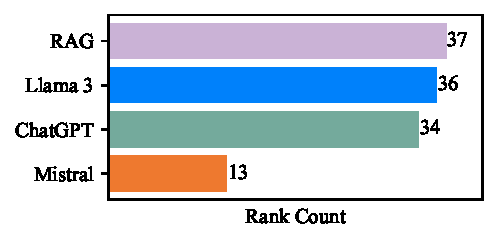
\includegraphics[width=\linewidth]{rank_count_final.pdf}
    \caption{
        Final Borda count scores. RAG model is the best, with Llama $3$
        and ChatGPT close behind. Mistral in many cases performs the
        worst.
    }
    \label{fig:fin_count}
\end{figure}

\section*{Discussion}

The results of our study highlight the varying strengths and weaknesses of the different models in the context of roleplaying, factuality, and engagement.
The latest open-source models, particularly Llama 3, have shown themselves to be competitive alternatives to proprietary models like ChatGPT. However, Mistral performed poorly across all criteria. In our testing, we found that
prompt engineering is not very effective for it. The initial prompt does make
the model mimic the character, but further changes to the prompt, do
not yield much of an improvement.

Since a lot of LLMs are trained on famous books like Harry Potter and Lord
of the Rings, along with internet discussions about them, they perform well on such topics. Still, all models make mistakes, especially on lesser-known
works, e.g., Alamut by Vladimir Bartol. Here, only the RAG model was factually
correct.

On other books, the RAG model was the most factual as well, but the information
retrieved with RAG can get in the way of authentic roleplay and sometimes 
feels more artificial than the other models. Nonetheless, the combination of
Llama 3 and RAG proved to be the best across the board, with the highest total
score of $37$.

We found that by using the right system prompt, we can make the models respond with engaging questions that promote critical thinking and deeper reflections in users, but even with the best prompt, the model can still skip proving
a question.

A promising direction for future work is to explore the use of various pedagogical techniques to further improve the educational value of the conversations students have with the persona bots. This could include personalized feedback to cater to individual learning styles and needs. Additionally, incorporating gamification elements and interactive storytelling could make the learning experience more engaging and immersive, fostering a deeper connection with the material.

%------------------------------------------------

%----------------------------------------------------------------------------------------
%	REFERENCE LIST
%----------------------------------------------------------------------------------------
\bibliographystyle{unsrt}
\bibliography{report}

\end{document}
